
\graphicspath{{Chapter2/Figs/}}

\setcounter{chapter}{5}
\chapter*{Capítulo 2} 
\addcontentsline{toc}{chapter}{Capítulo 2}
\setcounter{figure}{0}
\setcounter{section}{0}

{\LARGE Estudios genómicos sobre la biogénesis de precursores de miARN en plantas}


\section{Introducción}
Los miARNs son una clase de ARNs de 20-22nt de largo que son originados de genes endógenos y regulan otros ARNs por complementariedad de bases \citep{Voinnet2009669}.
Se distinguen de otros ARNs pequeños por su biogénesis única que involucra el corte preciso del precursor, para liberar el miARN maduro.
Aunque la evidencia actual indica que los miARNs han surgido y especializada de forma independiente en animales y las plantas, su biogénesis depende del reconocimiento de claves estructurales ubicadas en los precursores de miARN \citep{pmid21554756,citeulike:8816489,Bologna11112012}.

En nuestro grupo actualmente se está estudiando la biogenesis de miARNs, específicamente como los precursores son reconocidos y procesados en plantas \citep{Bologna2013}.
Estos precursores tienen una estructura de tallo-burbuja característica \citep{Jones-Rhoades2006}, que se cree que proporciona las claves para el procesamiento del mismo y la liberación de los ARN pequeños de 21 nt.

Mientras que los precursores de miARN en animales tienen estructuras homogéneas, los precursores de miARNs en plantas constituyen una amplia gama de estructuras, y sus longitud pueden variar entre 50 y 900 nucleótidos \citep{Bologna2013,citeulike:8816489}.
Esa variabilidad se da entre distintas familias de precursores, pero a veces también entre una misma familia de precursores en distintas especies (Figura \ref{fig:hairpin_distribution}).

Además, en las plantas, las mutaciones que impiden la biogénesis o actividad de los miARNs, tales como \textit{hyl1}, \textit{hen1} y \textit{ago1}, conducen al aumento en los niveles de los transcriptos de muchos de los genes blanco de miARNs (aproximadamente un 45\% de todos los blancos) \citep{Han2004,pmid12747833,pmid16889646,Allen2005207}.
Esto sugiere que el mecanismo que involucra el corte y degradación de los ARNm es un componente importante de la represión inducida por los miARNs en plantas \citep{Jones-Rhoades2006, Voinnet2009669}.

\begin{figure}[htbp!] 
    \centering    
    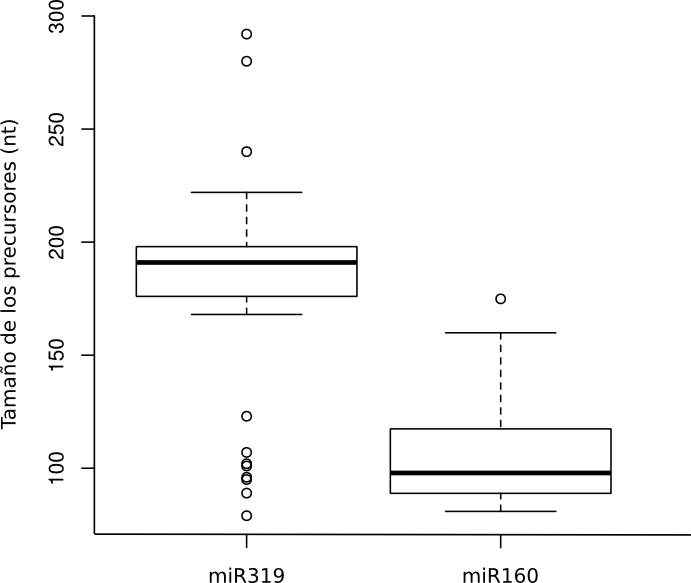
\includegraphics[width=.7\textwidth]{hairpin_distribution.png}
    \caption[Tamaño de precursores]{Tamaño de precursores. Se muestra el tamaño (nt) de dos familias de precursores en distintas especies.}
    \label{fig:hairpin_distribution}
\end{figure}

En particular, la biogénesis de los miARNs es un proceso clave porque determina la secuencia exacta de nucleótidos del ARN pequeño funcional.
Si bien en el caso de animales está claro cuáles elementos estructurales son reconocidos en los precursores durante su procesamiento, poco se sabía sobre el reconocimiento de los precursores de plantas por la maquinaria de procesamiento.

Muchos precursores en plantas tienen un tallo de $\sim$15 nt debajo del duplex miARN/miARN* seguido por un loop interno, que sirve como una señal estructural de reconocimiento por la maquinaria de procesamiento \citep{pmid17369351,pmid16751099,Mateos2010,pmid20015654}.
Sin embargo, este determinante de procesamiento no se encuentra en todos los precursores \citep{Mateos2010}.
Además, la biogénesis de los miARNs conservados evolutivamente como ser el miR319 y miR159 comienzan con un corte al lado del loop interno y continúa con 3 cortes adicionales en una dirección de burbuja a base hasta que finalmente el miARN es liberado \citep{Bologna2013,pmid19850910}.
Se ha demostrado que otros precursores de plantas liberan otros ARNs pequeños además del miARN \citep{pmid15314213,pmid20696037}, aunque los mecanismos de procesamiento subyacentes eran desconocidos.

\section{Resultados y Discusión}

%~ ################################################# 
%~ Procesamiento de precursores de miARNs en plantas
%~ #################################################

\subsection{Procesamiento de precursores de miARNs en plantas}
\label{sec:procesamiento}

En esta parte del proyecto de tesis y en el marco de una colaboración con el grupo del Dr. Blake Meyers (Delaware,USA), el cual se especializa en secuenciación y análisis de ARN pequeños, nos propusimos entender cómo se procesan los precursores de miARNs plantas. 
Colegas del laboratorio realizaron una estrategia para analizar sistemáticamente intermediarios de procesamiento de miARNs y caracterizar la biogénesis de la mayoría de los miARNs conservados presentes en \textit{A. thaliana} mediante técnicas de secuenciación de alto rendimiento, utilizando los equipos de última generación disponibles en Delaware (USA).
Esta técnica desarrollada en el laboratorio se conoce como SPARE \citep{Schapire2013} (del inglés Specific Parallel Amplification of RNA Ends).
Utilizando esta técnica encontramos que los miARNs son procesados por cuatro mecanismos, dependientes de la dirección secuencial de la maquinaria de procesamiento y del número de cortes requeridos para liberar el miARN.
La clasificación de los precursores, teniendo en cuenta los mecanismos de procesamiento, reveló determinantes estructurales específicos para cada grupo.
Se encontró que la complejidad de las vías de procesamiento de miARN se produce tanto en precursores jóvenes como en conservados y que los miembros de la misma familia pueden ser procesados de diferentes maneras.
Además hemos observado que diferentes determinantes estructurales compiten por la maquinaria de procesamiento y que miARNs alternativos pueden ser generados a partir de un único precursor.
Los resultados ofrecen una explicación para la diversidad estructural de los genes de precursores de miARN en plantas y nuevas perspectivas hacia la comprensión de la biogénesis de los ARNs pequeños \citep{Bologna2013}.


\subsubsection{Análisis de datos y precursores detectados}
Mediante la cantidad de cortes detectados la técnica de SPARE permite definir si el mecanismo es base a loop o loop a base.
Esta técnica arroja una gran cantidad de datos producto de la secuenciación de alto rendimiento, por lo que se necesita de un enfoque bioinformático para la interpretación de los resultados.
Por la gran cantidad de precursores a estudiar y el número de bibliotecas se necesitó un análisis previo de los datos y una forma de presentarlos.
Para esto construimos e implementamos un pipeline bioinformático utilizando "in-house" scripts y datos disponibles de miRBASE para poder analizar los datos de las bibliotecas de deep-sequencing obtenidos a partir de la técnica de SPARE.

Un precursor fue considerado como detectado si más de tres lecturas corresponden a la secuencia de ese precursor.
De esta manera encontramos fragmentos de ARN que corresponden a 129 precursores, 71 de ellos de miARNs conservados y 58 de miARNs jóvenes (Figura \ref{fig:GR_fig1C}).
Mediante el análisis de los datos arrojados de la estrategia bioinformática pudimos definir la dirección de procesamiento de la mayoría de los precursores en \textit{A. thaliana}.
De los cuales 32 de ellos fueron definidos como procesados por un mecanismo de base a loop, ya que se encontraron los cortes en la parte proximal del duplex miARN/miARN* sin detectar cortes en la parte de arriba del duplex, como en el caso del miR168a, miR172b y el miR395b (Figura \ref{fig:GR_fig2A}).
Además encontramos 16 precursores de miARNs conservados con cortes detectados (>5\%) en el lado distal del miARN/miARN* los cuales fueron definidos como loop a base (Figura \ref{fig:GR_fig4A}).

\begin{figure}[htbp!] 
    \centering    
    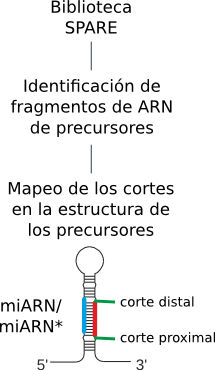
\includegraphics[width=.5\textwidth]{GR_fig1C.png}
    \caption[Esquema del procedimiento para analizar los datos de SPARE]{Esquema del procedimiento para analizar los datos de SPARE.}
    \label{fig:GR_fig1C}
\end{figure}

\begin{figure}[htbp!] 
    \centering    
    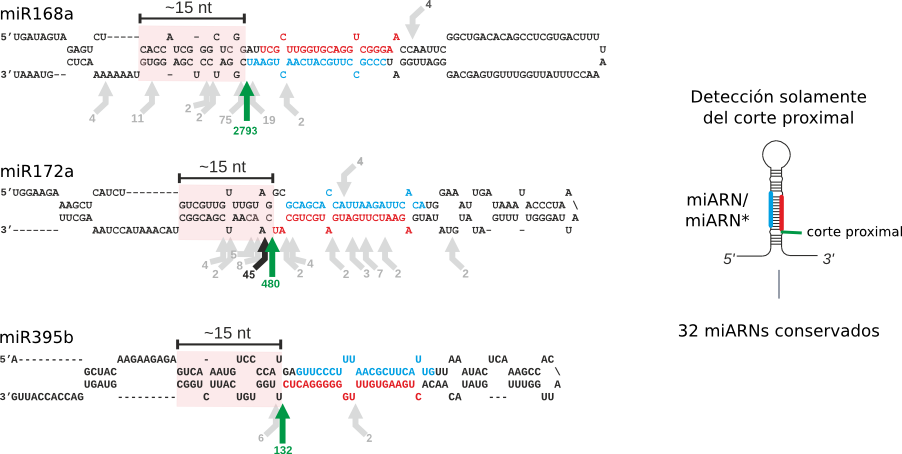
\includegraphics[width=.8\textwidth]{GR_fig2A.png}
    \caption[Identificación y caracterización de precursores de miARNs procesados de base a loop]{Identificación y caracterización de precursores de miARNs procesados de base a loop.
            Esquema donde se muestra la estructura secundaria del miR168a, miR172b y miR395b.
            Las flechas indican la posición y número de lecturas de los cortes del precursor identificado.
            Flechas en verde muestra el corte más abundante, que también coincide con al corte proximal del miARN/miARN*.
            Flechas en negro muestran otros cortes con al menos 5\% de abundancia del número total de cortes, mientras que otros cortes minoritarios se muestran con una flecha gris.
            Con rosa se resalta el stem de 15nt debajo del corte proximal.
            El miARN se indica en color rojo y el miARN* en color azul.
            La imagen de la derecha muestra el patrón de corte típico detectado en la biblioteca de SPARE para estos precursores.}
    \label{fig:GR_fig2A}
\end{figure}

\begin{figure}[htbp!] 
    \centering    
    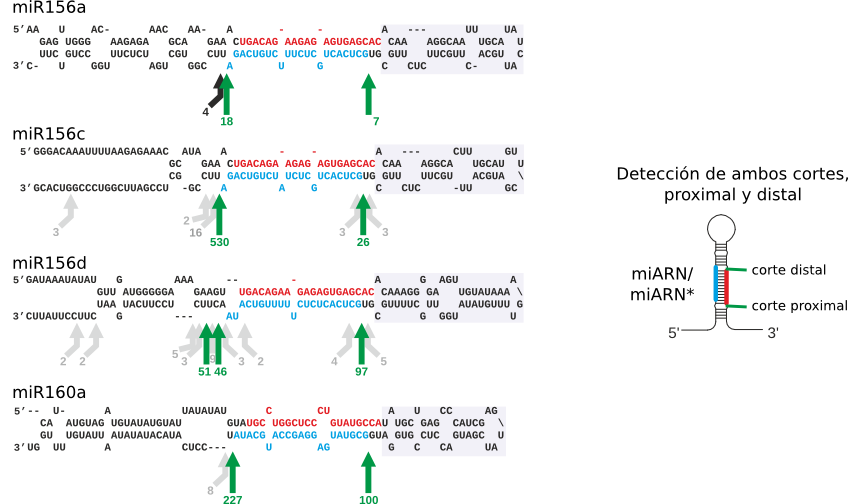
\includegraphics[width=.8\textwidth]{GR_fig4A.png}
    \caption[Identificación y caracterización de precursores de miARNs procesados de loop a base]{Identificación y caracterización de precursores de miARNs procesados de loop a base. 
    Esquema donde se muestra la estructura secundaria del miR156a, miR156c, miR156d y miR160a.
    Las flechas indican la posición y número de lecturas de los cortes del precursor identificado.
    Flechas en verde muestra el corte más abundante, que también coincide con al corte proximal del miARN/miARN*.
    Flechas en negro muestran otros cortes con al menos 5\% de abundancia del número total de cortes, mientras que otros cortes minoritarios se muestran con una flecha gris.
    Con gris se resalta el stem de arriba del miR156 y miR160. El miARN se indica en color rojo y el miARN* en color azul.
    La imagen de la derecha muestra el patrón de corte típico detectado en la biblioteca de SPARE para estos precursores.
}
    \label{fig:GR_fig4A}
\end{figure}

\subsubsection{Estructura secundaria de los precursores}
Para ver si había diferencias estructurales para los precursores con diferentes mecanismos de procesamiento, determinamos la estructura secundaria de precursores detectados que se procesan en dirección base a loop (Figura \ref{fig:GR_fig2C}) y los que se procesan loop a base (Figura \ref{fig:GR_fig4C}).
Obtuvimos las estructuras secundarias para cada precursor.
Definimos a una coincidencia en cada posición con un 0, mientras que "bulges" y "mismatches" los consideramos como 1.
El lado proximal del duplex miARN/miARN* fue definido como la posición +1 y analizamos desde la posición -25 a la posición +40 (Figura \ref{fig:GR_fig2C} y \ref{fig:GR_fig4C}). 

\subsubsection{Procesamiento de base a loop}

Consideramos la estructura secundaria de 32 precursores analizados en esta parte del trabajo que se procesan de base a loop y todos ellos tienen un claro tallo inferior de 15 nt de largo (Figura \ref{fig:GR_fig2C}).
Además este tallo se pudo ver tanto para los precursores validados experimentalmente que se procesan de base a loop como para todos los precursores conservados (Figura \ref{fig:GR_fig2C} en violeta).
Pero pudimos observar que las bases inmediatamente debajo del duplex miARN/miARN* (posición -2 y -1) tienden a estar desapareadas (Figura \ref{fig:GR_fig2C}).
Además las posiciones -3 y -4 y las 3 últimas posiciones del stem inferior (-13,-14 y -15) están apareadas casi siempre (Figura \ref{fig:GR_fig2C}).
En general, nuestros resultados muestran que los precursores procesados en una dirección base a loop son más uniformes de lo que se pensaba previamente y que al menos algunos de los precursores no detectados como base a loop probablemente tengan otros determinantes específicos de ARN.

\subsubsection{Procesamiento de loop a base}
Estos precursores, que tienen un procesamiento loop a base, tienen un corte mayoritario que se puede detectar en nuestras bibliotecas.
Este corte es el esperado en la dirección de procesamiento de precursores con un mecanismo de loop a base.
Con la excepción de dos miARNs (miR396a y miR162b) estos precursores no tienen una estructura obvia debajo del duplex miARN/miARN* (Figura \ref{fig:GR_fig4C}).
Estos precursores tienen una región terminal estructurada (Figura \ref{fig:GR_fig4C}), que tiene un tamaño homogéneo de ~42nt que incluye un loop corto en contraste con la misma región en los precursores que se procesan de base a loop donde es más variable (Figura \ref{fig:GR_fig2C} y \ref{fig:GR_fig4C}). 

En esta segunda parte del proyecto de tesis presentamos un estrategia y realizamos un análisis sistemático para la identificación de la biogénesis de precursores de miARNs desde un punto de vista genómico.
De esta manera pudimos encontrar la dirección de procesamiento de la mayoría de los precursores de miARNs en \textit{A. thaliana}.

\begin{figure}[htbp!] 
    \centering    
    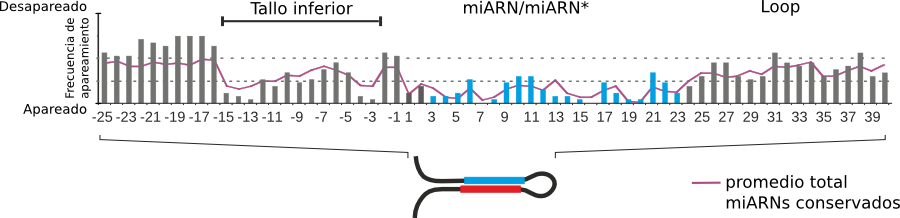
\includegraphics[width=1\textwidth]{GR_fig2C.png}
    \caption[Estructura secundaria de precursores de base a loop]{Estructura secundaria de precursores detectados que se procesan en dirección base a loop.
    Los matches en cada posición los consideramos como 0, mientras que "bulges" y "mismatches" fueron considerados como 1.
    La estructura secundaria considerando todos los miARNs conservados se indica con color violeta.
    }
    \label{fig:GR_fig2C}
\end{figure}

\begin{figure}[htbp!] 
    \centering    
    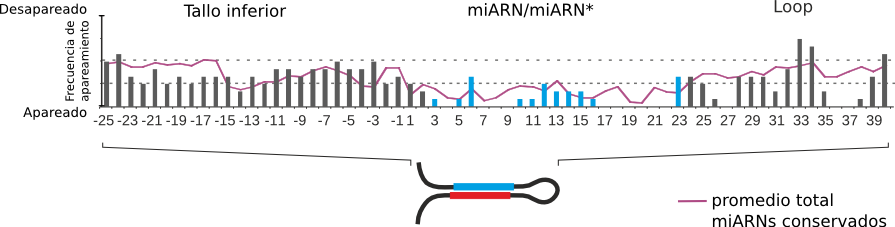
\includegraphics[width=1\textwidth]{GR_fig4C.png}
    \caption[Estructura secundaria de precursores de loop a base]{
    Estructura secundaria de precursores detectados que se procesan en dirección loop a base.
    Los matches en cada posición los consideramos como 0, mientras que "bulges" y "mismatches" fueron considerados como 1.}
    \label{fig:GR_fig4C}
\end{figure}


Estos resultados fueron publicado en la revista Genome Research \citep{Bologna2013}.
En este mismo artículo se pudo demostrar que los precursores de miARNs en plantas, se pueden agrupar por cuatro mecanismos de procesamiento con distintas características (Figura \ref{fig:mecanismos}).

\begin{itemize}
    \item En los precursores con un mecanismo \textbf{corto de base a loop}, un loop interno seguido por un tallo inferior de $\sim$15nt especifica la posición del primer corte.
        Esta estructura se encuentra en la mayoría de familias de miARNs \citep{Mateos2010,pmid20015653,pmid20015654}.
        A pesar de que el tallo puede contener bulges, la transición de un loop interno (simple hebra) al tallo inferior es bastante marcada, y tres pares de bases apareadas generalmente definen el comienzo del tallo inferior del precursor \citep{Bologna2013}.
        El segundo corte procede a una distancia fija de $\sim$21 nt desde la posición del primer corte.
    \item En los precursores con un mecanismo \textbf{secuencial de base a loop} (ej: familia del miR169), el primer corte procede como en los cortos de base a loop, pero luego son necesario dos cortes más para liberar el miARN, generando en el proceso niveles bajos de RNA pequeños adicionales \citep{Bologna2013}.
    \item En los precursores con un mecanismo \textbf{cortos de loop a base} (ej: familia del miR156 y miR160), el procesamiento es guiado por un tallo superior, y son necesarios dos cortes para liberar el miARN maduro.
        La región terminal de estos precursores tienen una largo conservado de $\sim$42 donde incluye un loop pequeño \citep{Bologna2013}.
    \item En los precursores con un mecanismo \textbf{secuencial de loop a base} (ej: familia del miR319 y miR159), cuatro cortes secuenciales por DCL1 son los encargados de procesar los precursores de miARNs.
        En general muestran un tallo largo superior, del cual otros ARNs pequeños son generados \citep{pmid19850910,Bologna2009,Bologna2013}
\end{itemize}

\begin{figure}[htbp!] 
    \centering    
    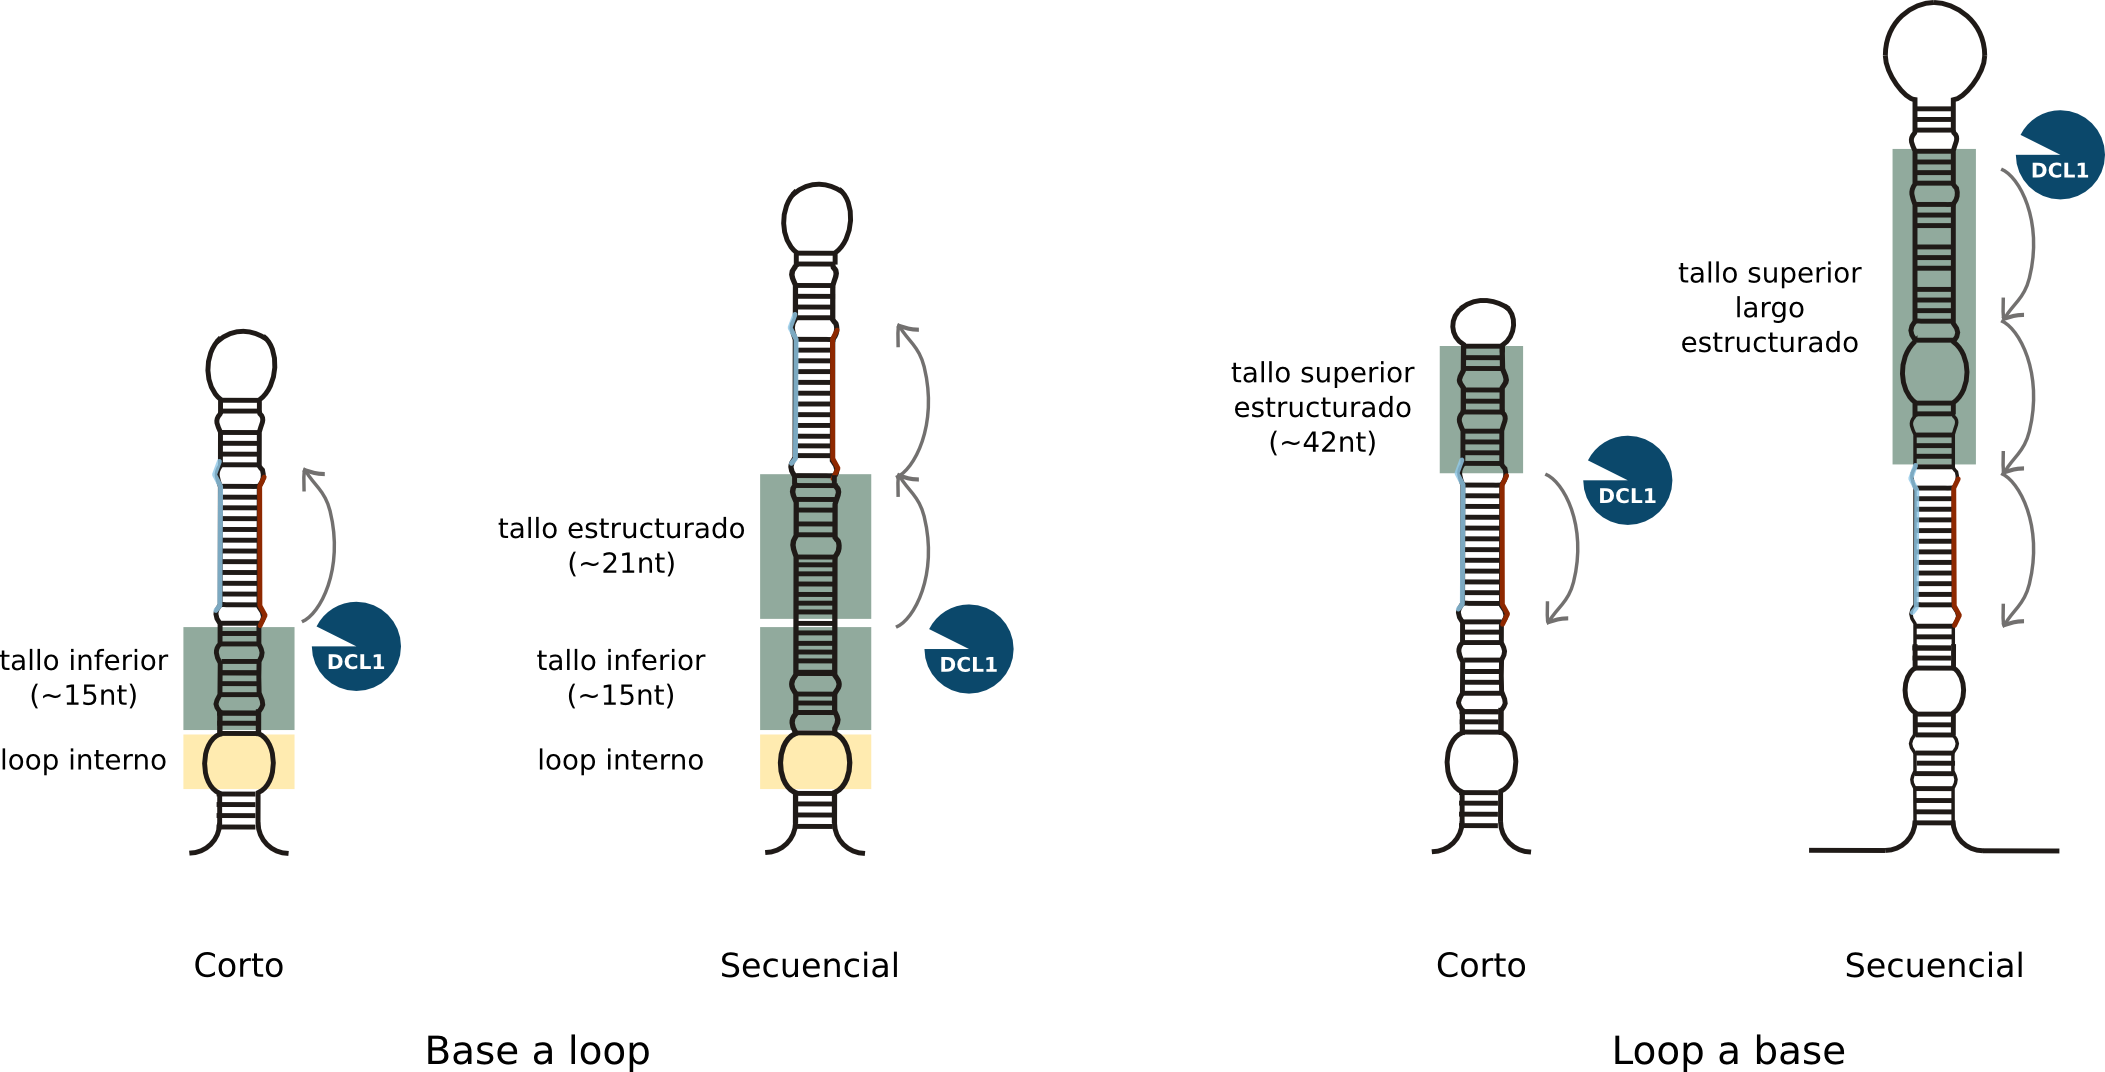
\includegraphics[width=1\textwidth]{mecanismos.png}
    \caption[Mecanismos de procesamiento]{Distintos mecanismos de procesamientos de miARNs en plantas}
    \label{fig:mecanismos}
\end{figure}


%~ ################################################# 
%~ Identificación de intermediarios de procesamiento
%~ en plantas mutantes en proteínas de procesamiento
%~ #################################################

\subsection{Identificación de intermediarios de procesamiento en plantas mutantes en proteínas de procesamiento}

La técnica de SPARE (del inglés Specific Parallel Analisys of 5'RNA Ends) fue desarrollada con el objetivo de caracterizar el procesamiento de los precursores de miARNs de \textit{A. thaliana}.
Para esto se identifican los intermediarios de procesamiento de cada uno de dichos precursores, y uniendo la información brindada por los diferentes fragmentos es posible dilucidar tanto la dirección, como el número de cortes requeridos para la biogénesis de cada miARN (Figura \ref{fig:SPARE_tecnica}).

\begin{figure}[htbp!] 
	\centering    
	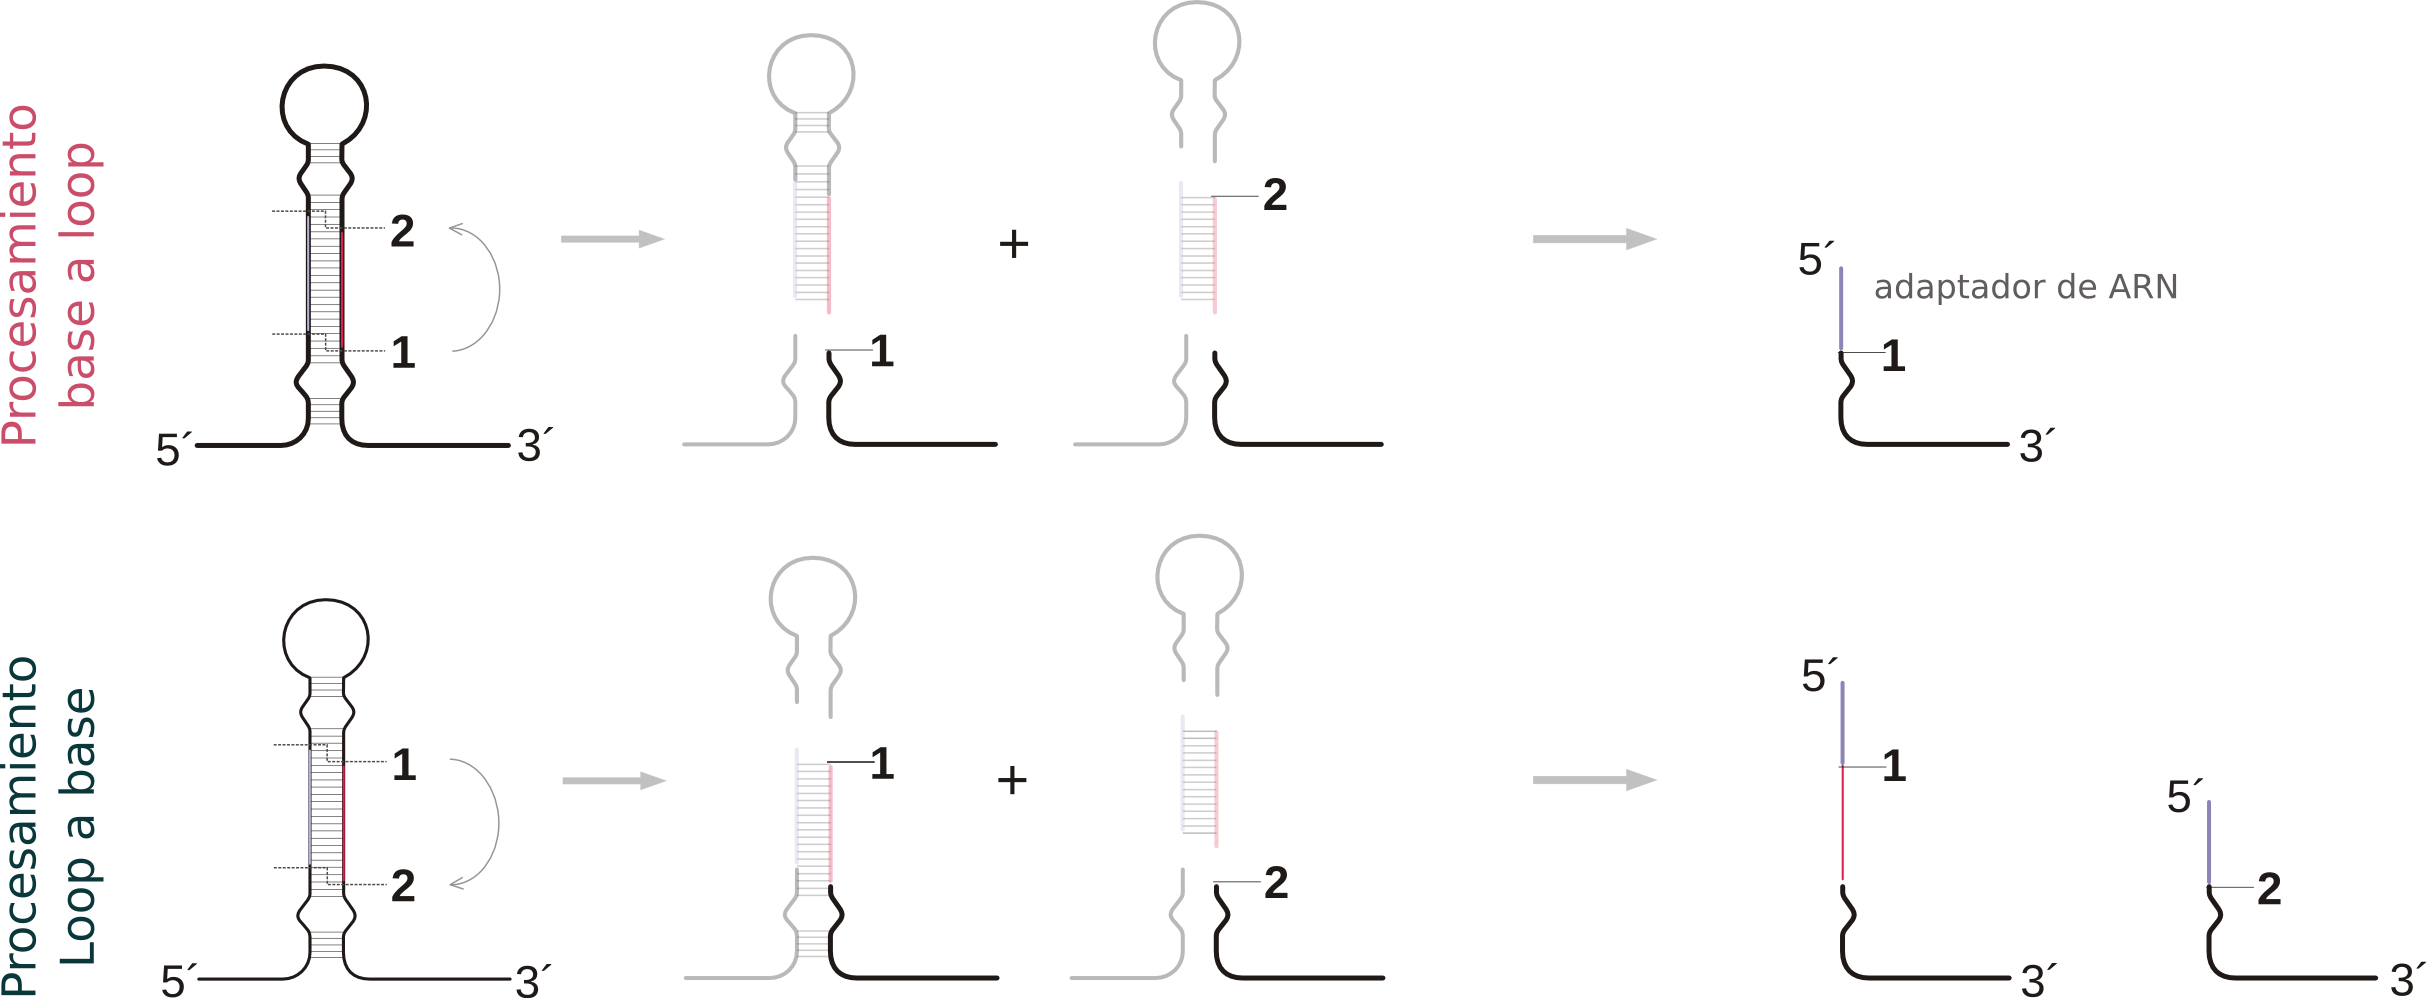
\includegraphics[width=1\textwidth]{SPARE_tecnica.png}
	\caption[Técnica de SPARE]{Técnica de SPARE para diferenciar mecanismos de procesamiento de precursores.
	Detalle donde se muestra a nivel molecular como la técnica permite diferenciar entre dos direcciones de procesamiento opuestas. }
	 \label{fig:SPARE_tecnica}
\end{figure}

Brevemente la técnica consiste en emplear los extremos 5'P dejados por la maquinaria de procesamiento en los precursores luego del clivaje para realizar una ligación ARN-ARN entre los intermediaros de procesamiento y un oligo de ARN de secuencia conocida.
A continuación se emplean oligos específicos para retro-transcribir los intermediaros de cada precursor en particular, con una cola común a todos.
En este punto todos los fragmentos generados durante el procesamiento presentan los mismos extremos: en el 5' la secuencia del oligo de ARN y el en el extremo 3' la secuencia común incorporada durante la retro-transcripción.
Esta información es empleada para diseñar oligos (FW y RV) que se emplean en una reacción de PCR a continuación.
Finalmente los fragmentos son secuenciados. 

En la sección \ref{sec:procesamiento} mostramos los resultados obtenidos de esta técnica para determinar la dirección de procesamiento de los precursores de miARNs en plantas.
Esta nueva secuenciación se realizó debido que anteriormente no se pudieron de determinar la dirección de procesamiento de algunos precursores.
Además, en esta nueva tanda de secuenciación de precursores se intentó identificar intermediarios de procesamiento en plantas mutantes en proteínas de procesamiento.  
Para esta parte del trabajo se hicieron algunas modificiaciones de la técnica.
Se ubicaron los oligos a 100 nt del último corte 3' esperado.
En total se diseñaron 121 oligos para retrotranscribir el conjunto de precursores conservados y jóvenes validados hasta el momento.  
Además, anteriormente el procesamiento de los datos a partir de los datos crudos se hicieron en el mismo laboratorio que se realizaron las secuenciaciones.

\subsubsection{Construcción de bibliotecas multiplex}
El paso final consiste en secuenciar las bibliotecas construidas, sin embargo la secuenciación es costosa haciendo económicamente dificultoso secuenciar varias bibliotecas en paralelo para comparar entre diferentes condiciones (siendo este nuestro objetivo con las plantas mutantes en proteínas de procesamiento).
En los últimos años se han desarrollado métodos que hacen posible secuenciar más de una biblioteca por calle.
Esto consiste en marcar los fragmentos provenientes de cada biblioteca con secuencias especificas (detallado en Materiales y Métodos) y separar informáticamente cada secuencia en la biblioteca de la cual provino a luego de secuenciación.
Técnicamente esto se hace agregando una PCR final donde los índex son incorporados en todas las secuencias de cada biblioteca.

\subsubsection{Diseño experimental}

Con el objetivo de construir bibliotecas de SPARE crecimos plántulas de Arabidopsis thaliana durante 10 días con luz continúa (independizándonos de este modo la variación asociada al ritmo circadiano a la hora de la colecta de muestra).
Se realizó un experimento con plantas mutantes en proteínas de procesamiento.

\textbf{Plantas mutantes en proteínas de procesamiento}

\textit{Hyl1}, \textit{Se} y \textit{Fiery}.
Siendo sus controles plantas silvestres de Arabidopsis ecotipo Col-O.

%~ \textbf{Plantas sometidas a diferentes temperaturas}
%~ 
%~ En este caso sólo se utilizaron plantas Col-0 y fiery crecidas en las condiciones descriptas anteriormente y que luego fueron sometidas a un tratamiento de dos horas a tres temperaturas diferentes: 8 \degree C, 22 \degree C y 37 \degree C.
%~ Luego se realizó la colecta de muestra a la temperatura del tratamiento. 

\subsubsection{Herramienta web para el análisis de intermediarios de procesamiento en plantas}

De la técnica de SPARE se obtienen una gran cantidad de datos arrojados por el secuenciador para cada biblioteca secuenciada.
Estos datos se conocen como datos crudos y son fragmentos de secuencia que luego tienen que ser mapeados contra el genoma de datos de interés.
Además, estos datos crudos cuentan con información de las secuencia, lo que permite mediante programas informáticos hacer un control de calidad de la secuencias obtenidas.
En total se obtuvieron cerca de 150 millones de secuencias (Figura \ref{fig:SPARE_estrategia}).

Esos fragmentos son agrupados y mapeados contra las secuencias únicas de los precursores de \textit{A. thaliana}.
Nos quedamos con 7158 secuencias únicas, que luego las filtramos por largo de la secuencia (Figura \ref{fig:SPARE_estrategia}).
Esa información ya procesada es la que utilizamos en la herramienta para analizar y comparar los intermediarios de procesamiento para plantas silvestreste y mutantes de procesamiento.

Para facilitar el análisis de los datos obtenidos por la técnica de SPARE, creamos una herramienta web disponible en la red interna del laboratorio.
La herramienta permite seleccionar un precursor en particular de los $\sim$100 precursores que se detectaron fragmentos por la técnica de SPARE.
Luego se selecciona una o varias mutantes y controles que se quieren analizar.
Además la herramienta permite modificar otros parámetros como la longitud y abundancia de los fragmentos secuenciados a considerar.

\begin{figure}[htbp!] 
	\centering    
	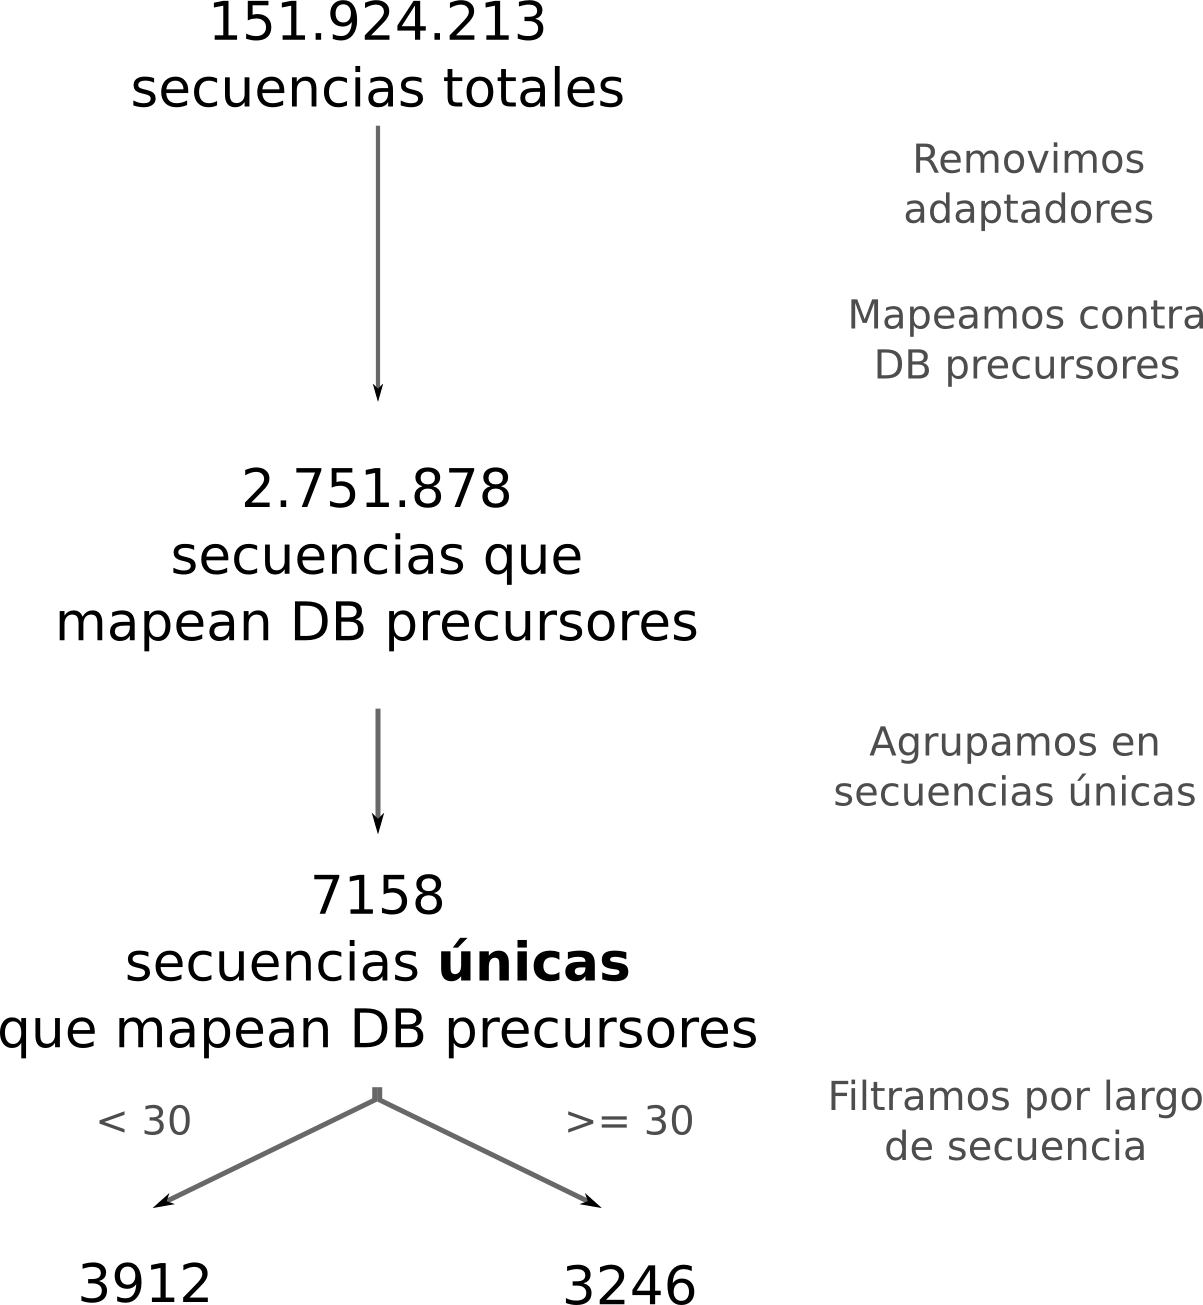
\includegraphics[width=.5\textwidth]{SPARE_estrategia.png}
	\caption[Análisis informático utilizado para procesar los datos de SPARE]{
	Análisis informático utilizado para procesar los datos de SPARE.
	Las secuencias únicas mapeadas contra los precursores son las que se utilizan en la herramienta para analizar los intermediarios de procesamiento.
	}
	 \label{fig:SPARE_estrategia}
\end{figure}

Primero vemos la salida de la herramienta para el precursor del  miR165a, analizando distintas mutantes de procesamiento al mismo tiempo (Figura \ref{fig:miR165a_SPARE}).
La posición final del duplex miARN/miARN* fue considerada como la posición 0, y las posiciones positivas son bases hacia arriba del dúplex mientrás que las posiciones negativas son bases hacia abajo del dúplex.
Los fragmentos se muestran en forma porcentual tomando cada biblioteca de forma independiente y en distintos colores se representan las distintas bibliotecas.
Además se muestra una tabla con los valores absolutos de cada fragmento y con flechas verdes se marcan las posiciones con los fragmentos de mayor abundancia en promedio de todas las bibliotecas (Figura \ref{fig:miR165a_SPARE}).
 
En esta figura se muestra un precursor que es procesado con un mecanismo corto de base a loop, donde según se muestra en la Figura \ref{fig:SPARE_tecnica}, los fragmentos detectados corresponden únicamente al primer corte por DCL1 (Figura \ref{fig:miR165a_SPARE}).
Se pueden observar también cortes en las posiciones $\pm 2$ con respecto a las esperadas por actividad "sloopy" (poco rigurosa) de DCL1 \citep{pmid17989254}.
Además se observan en la posición -5, que aparecen fragmentos en todas las bibliotecas aunque en muy baja abundancia (Figura \ref{fig:miR165a_SPARE}).

Mediante esta herramienta no sólo se puede identificar los precursores procesados de base a loop o de loop a base, sino que también permite identificar a los precursores que denominamos secuenciales, que son los que requieren de más de dos cortes por DCL1 para liberar al miARN maduro.
Por ejemplo, mostramos al precursor del miR169d que es procesado de forma secuencial de base a loop.
En estos precursores, los sitios de cortes delestán localizados 21 nt por debajo del lado proximal del dúplex miARN/miARN* y luego DCL1 sigue cortando para procesar al precursor.
En este caso se detecta un fragmento mayoritario en la posición -21, es decir 21nt por debajo del dúplex miARN/miARN* como era esperado para precursores secuenciales de base a loop \ref{fig:miR169d_SPARE}.

El precursor del miR169d tiene una estructura particular donde presenta un loop terminal ramificado.
Se ha estudiado este tipo de precursores, con esta estructura, donde se demostró que pueden ser procesados por DCl1 de manera bidireccional de base a loop o de loop a base, resultando en un procesamiento productivo y abortivo respectivamente \citep{pmid23934148}.
Con la herramienta desarrollada por nosotros, se puede observar que este precursor particular presenta fragmentos que provienen del corte secuencial de la base al loop que corresponde a la posición -21 en el gráfico.
Pero además, en la mutante de \textit{fiery} se pueden observar fragmentos que corresponden a un corte abortivo por DCL1 a partir del reconocimiento de este loop ramificado \ref{fig:miR169d_SPARE}.
La herramienta permite discriminar este tipo de procesamiento en distintas mutantes de procesamiento. 

\begin{landscape}
    \begin{figure}[htbp!] 
        \centering    
        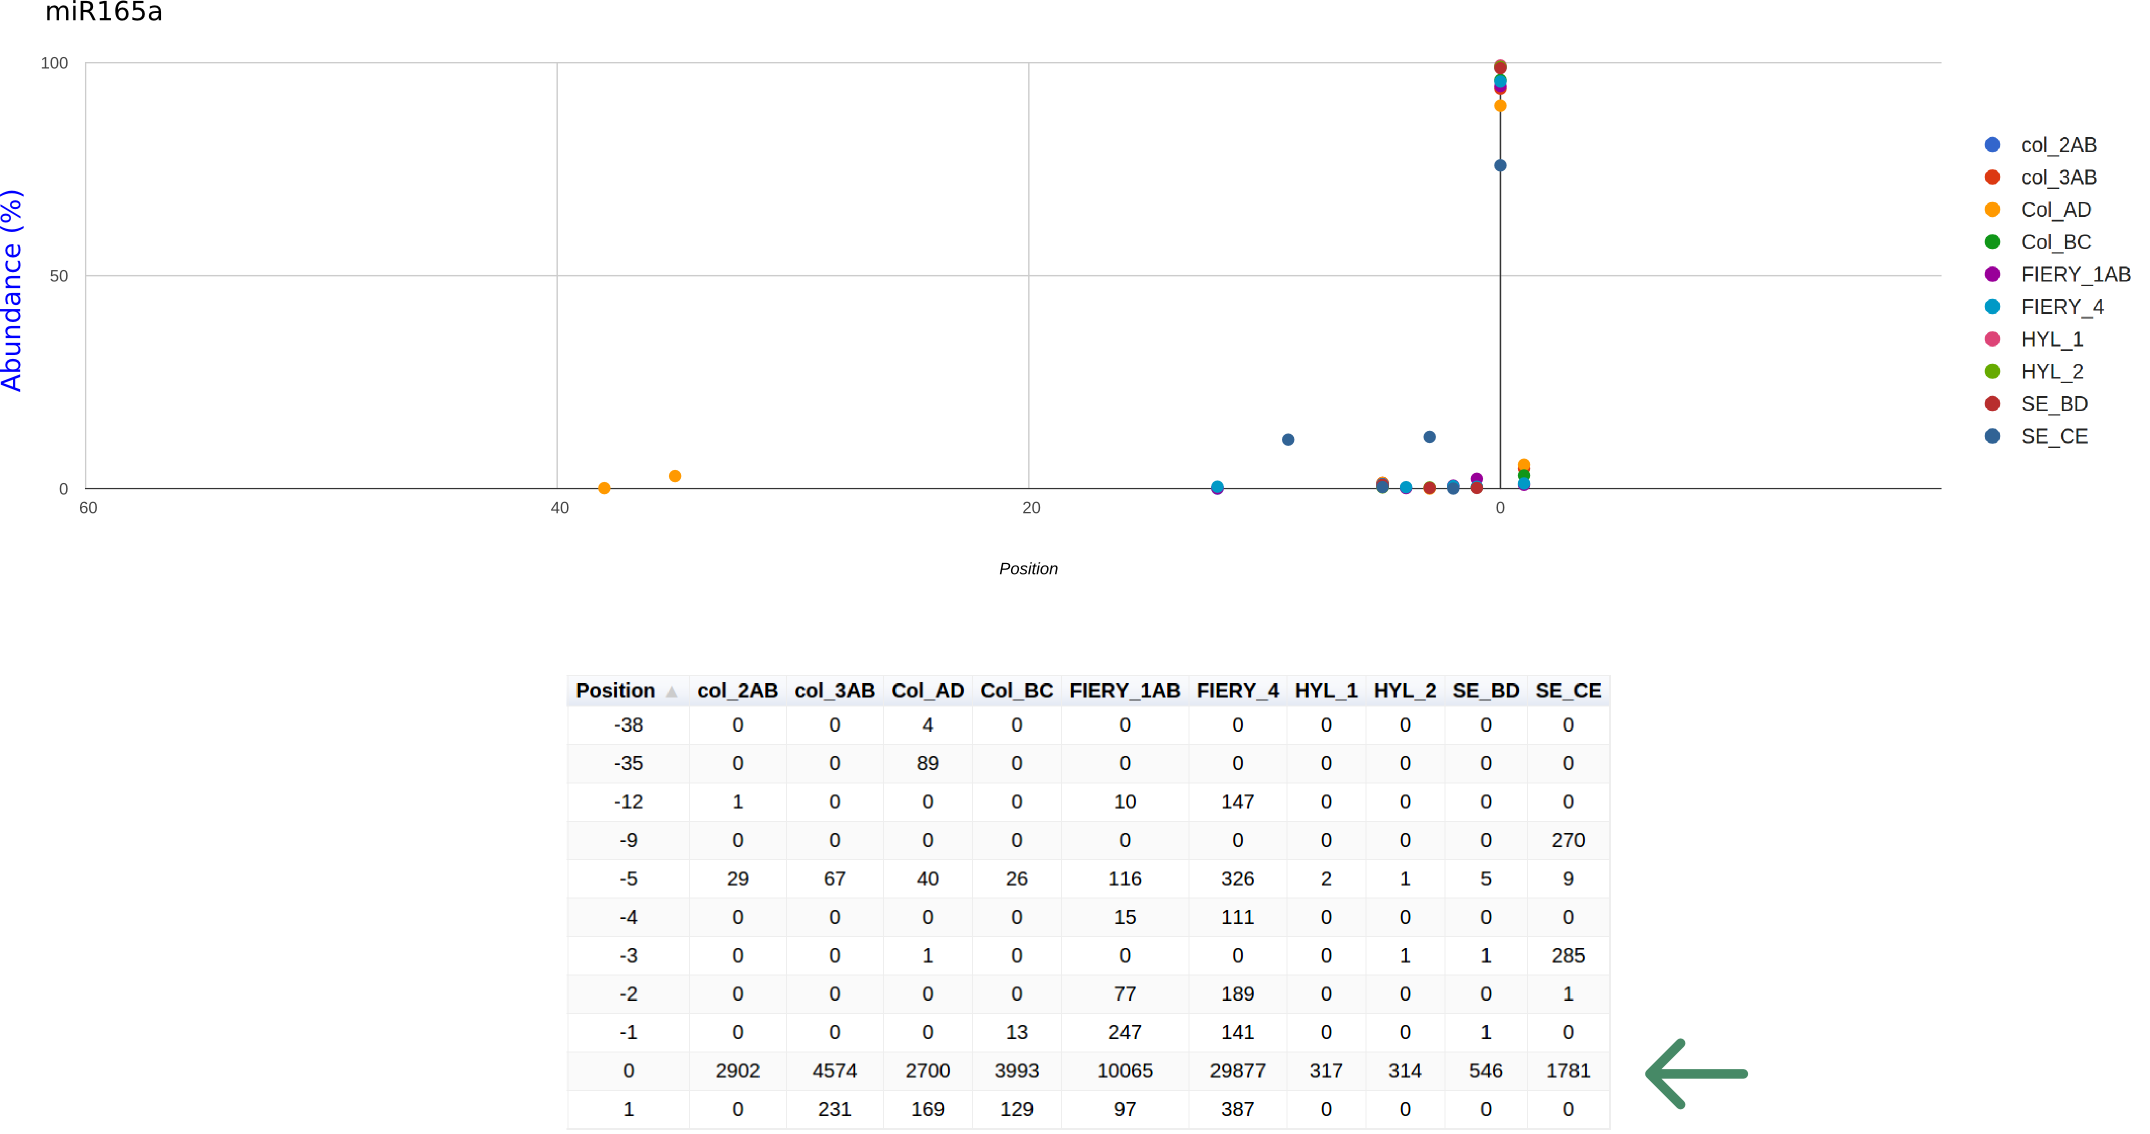
\includegraphics[width=1.4\textwidth]{miR165a_SPARE.png}
        \caption[Captura de pantalla de la herramienta de SPARE para el miR165a]{Captura de pantalla de la herramienta de SPARE para el miR165a.
        Porcentaje de fragmentos del precursor (abundancia relativa de los fragmentos en esa posición dividido la abundancia total de los fragmentos en el precursor).
        La posición final del duplex miARN/miARN* fue considerada como la posición 0.
        La tabla muestra los valores absolutos de cada fragmento.
        Las flechas verdes marcan las posiciones del precursor con los fragmentos de mayor abundancia. 
        }
         \label{fig:miR165a_SPARE}
    \end{figure}
\end{landscape}

\begin{landscape}                                                                      
\begin{figure}[htbp!] 
        \centering    
        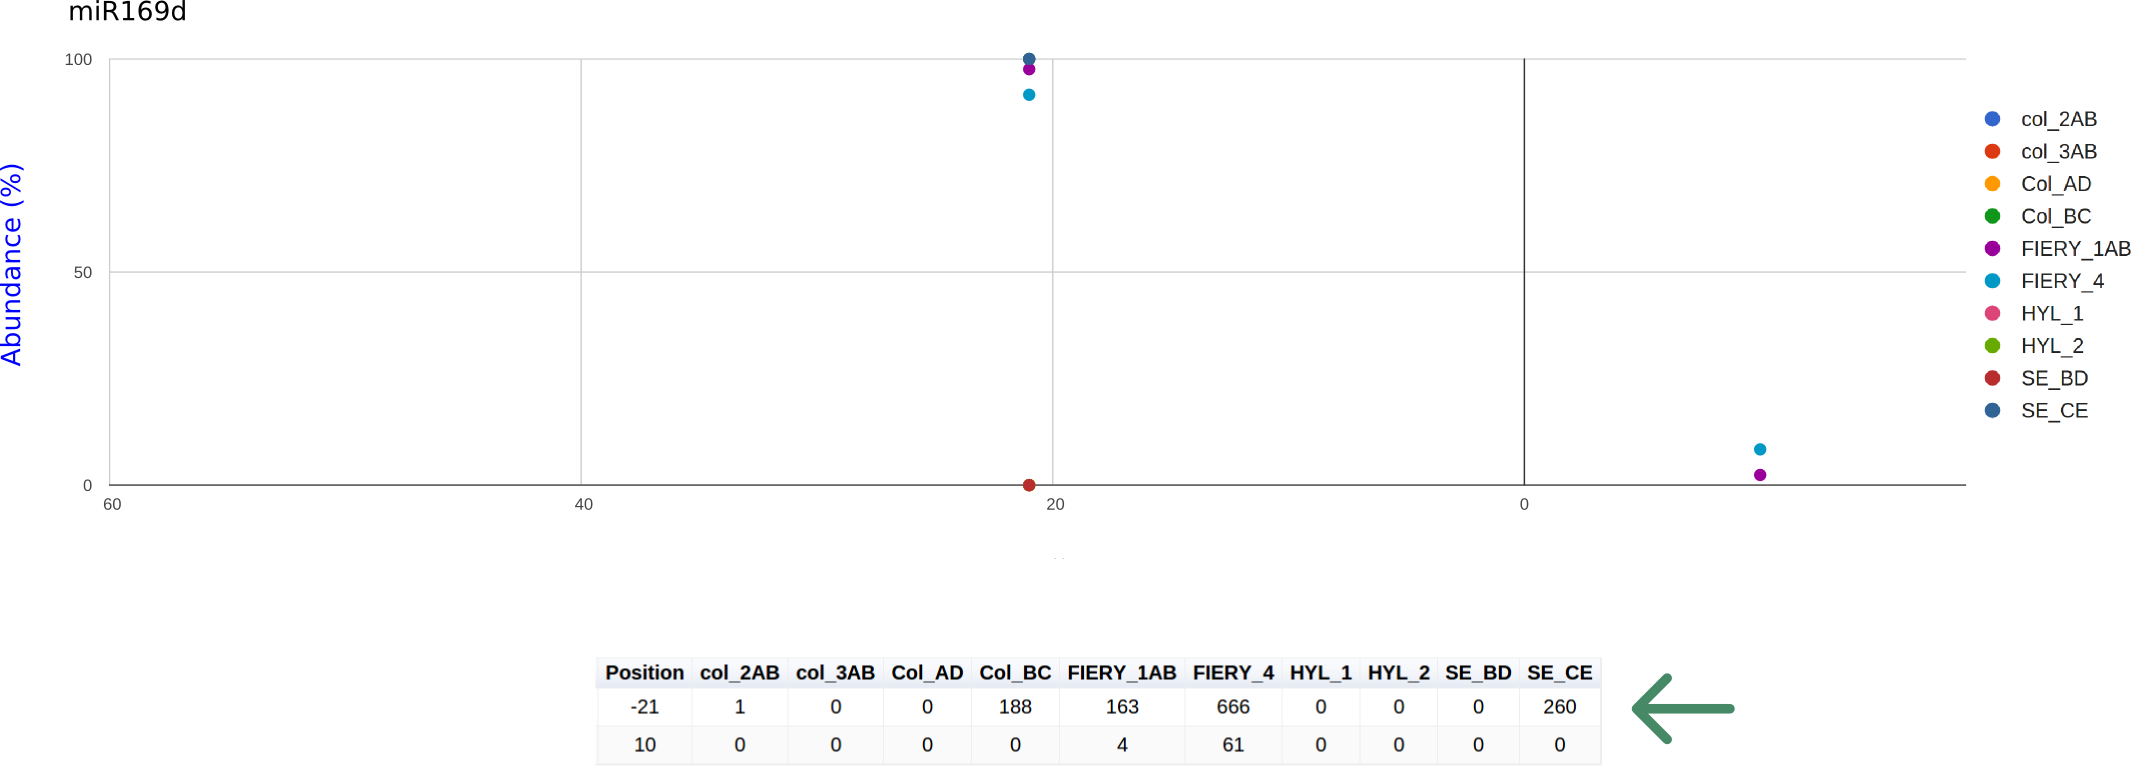
\includegraphics[width=1.4\textwidth]{miR169d_SPARE.png}
        \caption[Captura de pantalla de la herramienta de SPARE para el miR169d]{Capturntalla de la herramienta de SPARE para el miR169d.
        Porcentaje de fragmentos del precursor (abundancia relativa de los fragmentos eosición dividido la abundancia total de los fragmentos en el precursor).
        La posición final del duplex miARN/miARN* fue considerada como la posición 0.
        La tabla muestra los valores absolutos de cada fragmento.
        Las flechas verdes marcan las posiciones del precursor con los fragmentos de mayor abundancia. 
        }
	 \label{fig:miR169d_SPARE}
    \end{figure}
\end{landscape}

Para el caso de los precursores cortos de loop a base, los fragmentos detectados pueden ser más de uno según muestra la técnica de SPARE (Figura \ref{fig:SPARE_tecnica}).
Vemos el precursor del miR156a, donde los cortes más abundantes corresponden a las posiciones 22 y 0 (Figura \ref{fig:miR156a_SPARE}).
Estos fragmentos corresponden a los cortes del precursor por DCL1, donde el primer corte se da en la parte distal del dúplex y el segundo en la parte proximal del mismo.
Además se pueden observar otros fragmentos con abundancias relativas, cercanas a estas posiciones. 
En algunas bibliotecas se puede observar que acumulan más el primer corte (por ejemplo la biblioteca de Col\_AD) y en otras el segundo es el más abundate (biblioteca de Fiery\_1AB) (Figura \ref{fig:SPARE_tecnica}).
Esto podría ser interesante para estudiar en un futuro.
Además se puede observar que en \textit{Hyl} y \textit{Serrate} hay otros fragmentos con abundancia relativa en otras posiciones que las esperadas (posición 3 y posición 14 respectivamente), sugeriendo que tal vez que los cortes podrían estar afectados en estas mutantes de procesamiento (Figura \ref{fig:SPARE_tecnica}).

Por último en el caso del miR159, y al igual que todos los precursores que son procesados secuenciales de loop a base los cuatros fragmentos más abundantes corresponden a los cuatro cortes realizados por DCL1 que son requeridos para procesar este precursor (Figura \ref{fig:miR159b_SPARE}).
El primer corte se da en la posición 71, que de los cuatros cortes es el que tiene fragmentos menos abundantes, y luego DCL1 corta a 21 nucleótidos liberando otros ARN pequeños.
Luego se pueden observar los fragmentos correspondientes al tercer (posición 21) y cuarto corte (posición 0), que son los necesarios para liberar el miARN maduro (Figura \ref{fig:miR159b_SPARE}).
En este caso se pueden ver otros fragmentos que son productos de la degreadación del precursor, aunque nunca son tan abundantes como los fragmentos de los cortes por DCL1.
Por cuestiones de simplicidad, en la tabla solo se muestra los fragmentos con mayor abundancia en promedio de todas las bibliotecas.


\begin{landscape}
    \begin{figure}[htbp!] 
        \centering    
        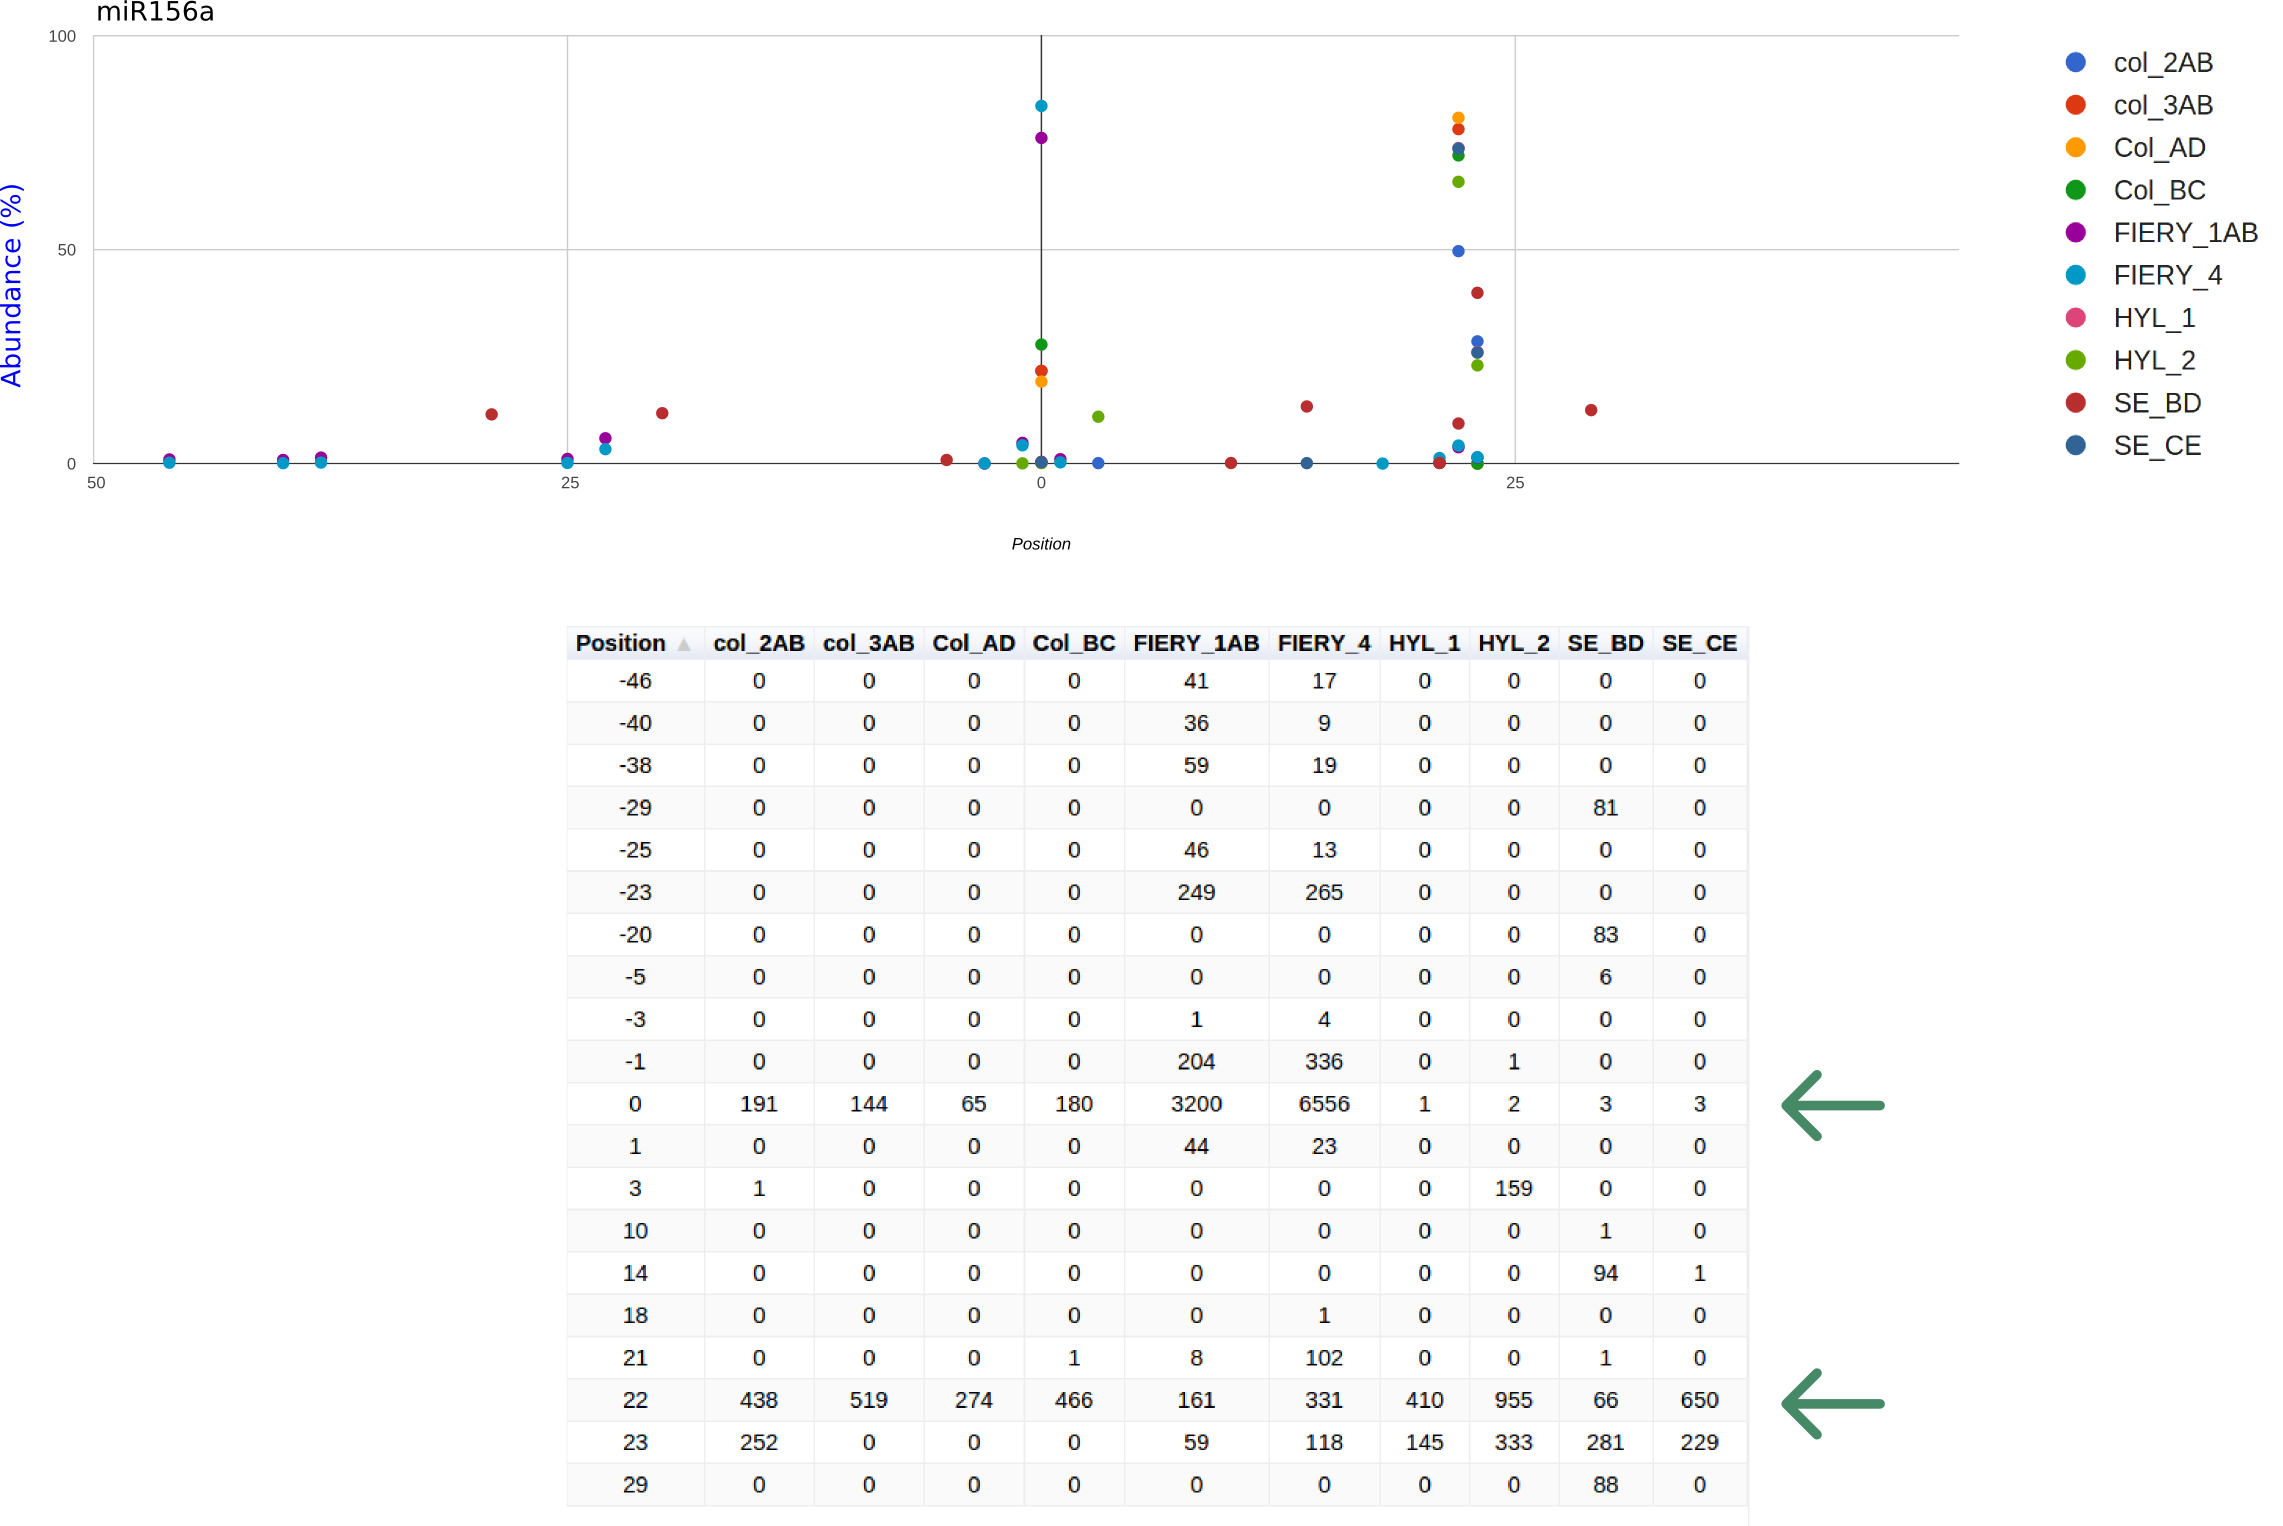
\includegraphics[width=1.4\textwidth]{miR156a_SPARE.png}
        \caption[Captura de pantalla de la herramienta de SPARE para el miR156a]{Captura de pantalla de la herramienta de SPARE para el miR156a.
        Herramienta para analizar los datos de la técnica SPARE.
        Porcentaje de fragmentos del precursor (abundancia relativa de los fragmentos en esa posición dividido la abundancia total de los fragmentos en el precursor).
        La posición final del duplex miARN/miARN* fue considerada como la posición 0.
        La tabla muestra los valores absolutos de cada fragmento.
        Las flechas verdes marcan las posiciones del precursor con los fragmentos de mayor abundancia. 
        }
         \label{fig:miR156a_SPARE}
    \end{figure}
\end{landscape}



\begin{landscape}
    \begin{figure}[htbp!] 
        \centering    
        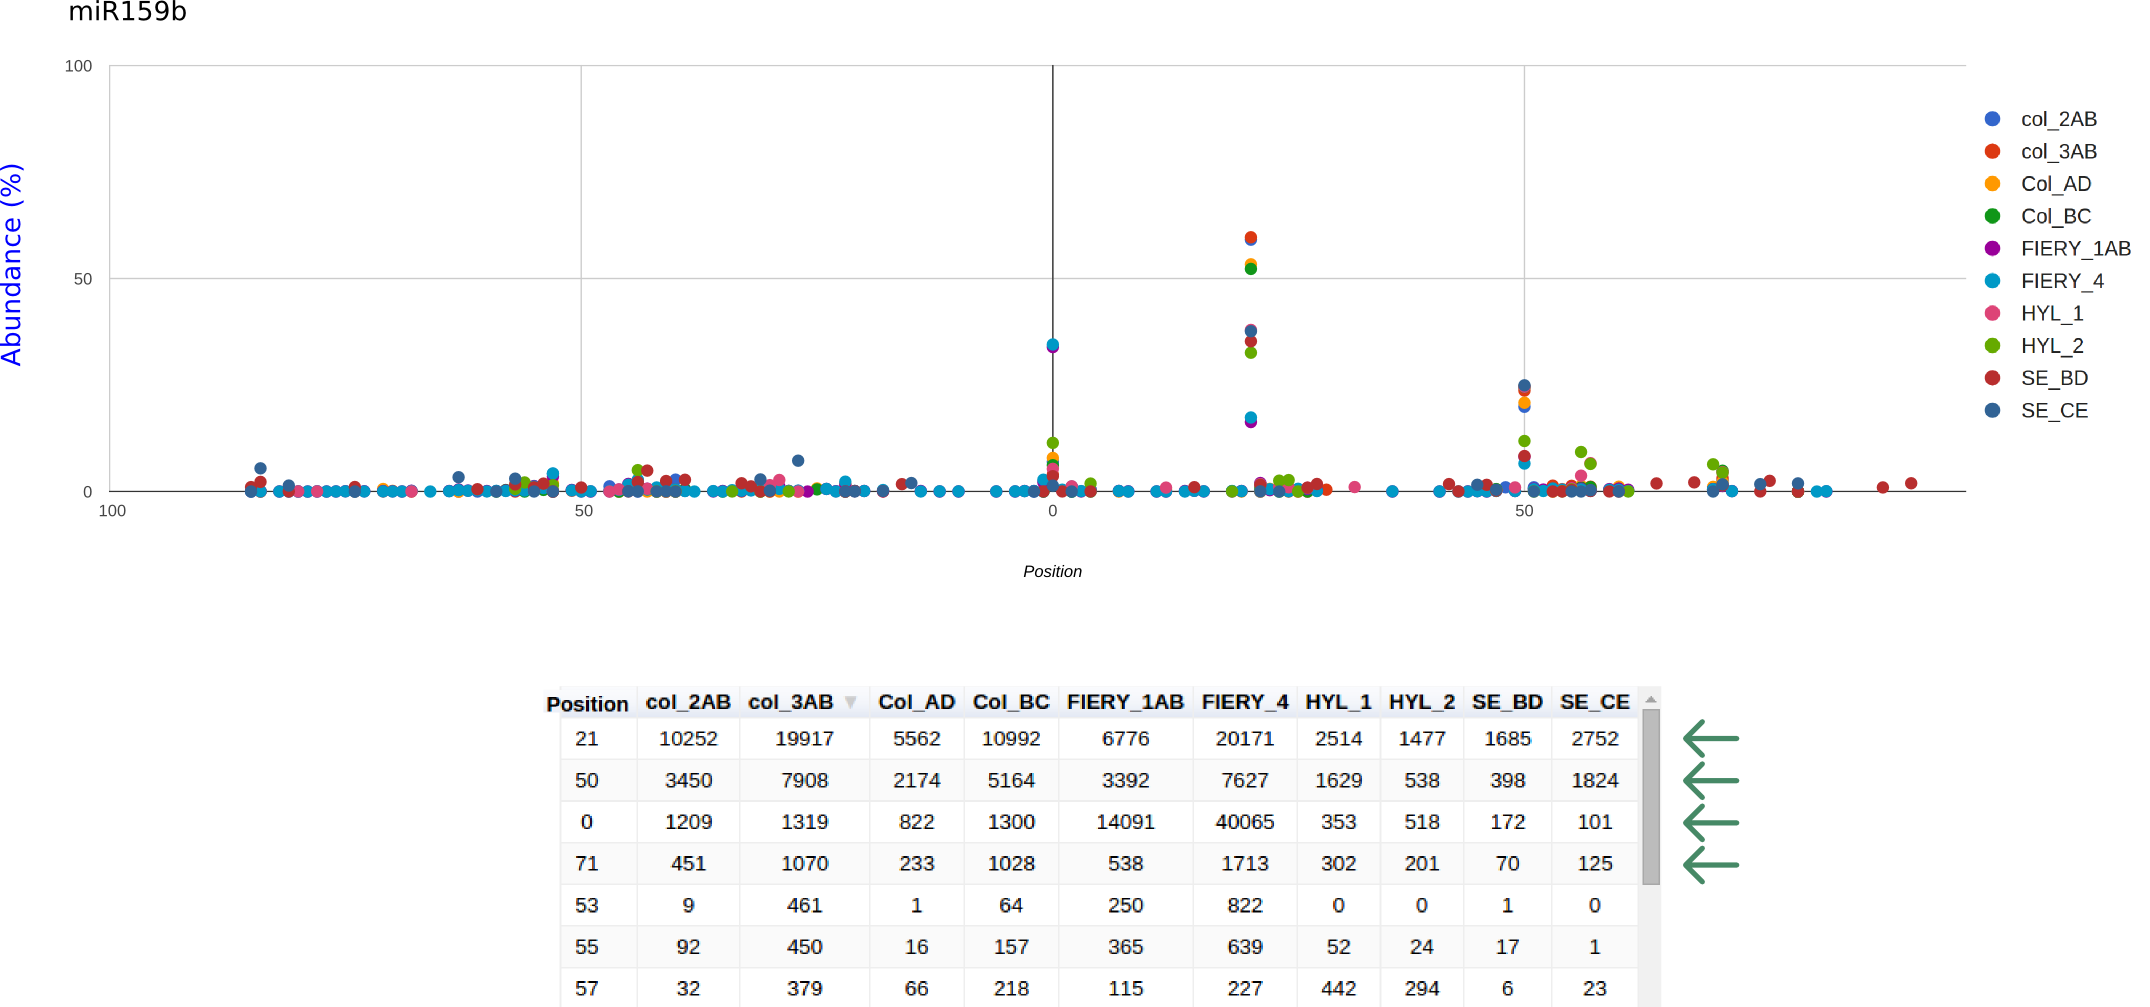
\includegraphics[width=1.4\textwidth]{miR159b_SPARE.png}
		\caption[Captura de pantalla de la herramienta de SPARE para el miR159b]{Captura de pantalla de la herramienta de SPARE para el miR159b.
        Porcentaje de fragmentos del precursor (abundancia relativa de los fragmentos en esa posición dividido la abundancia total de los fragmentos en el precursor).
        La posición final del duplex miARN/miARN* fue considerada como la posición 0.
        La tabla muestra los valores absolutos de cada fragmento.
        Por cuestiones de simplicidad, solo se muestran en la tabla los fragmentos con mayor abundancia en promedio de todas las bibliotecas.
        Las flechas verdes marcan las posiciones del precursor con los fragmentos de mayor abundancia.
        }
		\label{fig:miR159b_SPARE}
    \end{figure}
\end{landscape}


